\begin{exercise}
Figure \ref{fig:2.21} (below) gives the optimal value of the best state of the gridworld as $24.4$, to one decimal place.
Use your knowledge of the optimal policy and \eqref{eq:2.15} to express this value symbolically, and then to compute it to three decimal places.

\begin{figure}[H]
    \centering
    \subfloat[Gridworld]
    {
        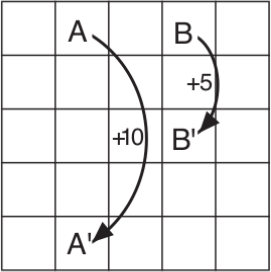
\includegraphics[width = 0.2 \textwidth]{2.21.1.png}
    }
    \hspace{1cm}
    \subfloat[$v_\ast$]
    {
        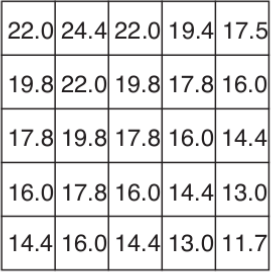
\includegraphics[width = 0.2 \textwidth]{2.21.2.png}
    }
    \hspace{1cm}
    \subfloat[$\pi_\ast$]
    {
        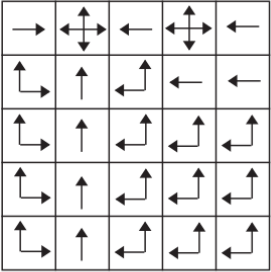
\includegraphics[width = 0.2 \textwidth]{2.21.3.png}
    }
    \hspace{0mm}
    \caption
    {
        Optimal solutions to the gridworld example.
    }
    \label{fig:2.21}
    \end{figure}
\end{exercise}

\begin{solution}
  Once we are in the best state $A$ and follow the optimal policy, we get a reward of $10$ for moving out of the state and then move up again, getting no reward for $4$ steps until we are in state $A$ again. With this we compute

  \begin{align*}
    v_*(A)
    &=
    \E_{\pi_*}\bigg[\sum_{k=0}^\infty \gamma^k R_{t+k+1}\mid S_t = A\bigg]
    =
    \sum_{k=0}^\infty \gamma^k \E_{\pi_*}\bigg[R_{t+k+1}\mid S_t = A\bigg] \\
    &=
    \sum_{k=0}^\infty \gamma^k \1_{\{k = 0 \mod 5\}} \cdot 10
    =
    10 \cdot \sum_{k=0}^\infty \big(\gamma^5\big)^k
    =
    \frac{10}{1-(0.9)^5}
    \approx
    24,4194
  \end{align*}
\end{solution}
